\chapter{Правила оформлення звіту}
\section{Титульна сторінка лабораторної роботи}
%\begin{titlepage}
%\newpage

\hrulefill

\begin{center}
МІНІСТЕРСТВО ОСВІТИ І НАУКИ, МОЛОДІ ТА СПОРТУ УКРАЇНИ \\

ХЕРСОНСЬКИЙ НАЦІОНАЛЬНИЙ ТЕХНІЧНИЙ УНІВЕРСИТЕТ \\*

КАФЕДРА ІНФОРМАЦІЙНИХ ТЕХНОЛОГІЙ

\end{center}

\vspace{5em}

\begin{center}
\Large Звіт до лабораторної роботи \No 123 \\ з дисципліни <<Web-програмування>>
\end{center}

\vspace{2.5em}

\begin{center}
{\Large Тема: \textbf{<<Основи мережі Internet>>}}
\end{center}

\vspace{5em}





\begin{flushleft}
Виконав \\ст.групи хПР1 \hspace{\fill} Пупкін А.А. \\
\vspace{1em}
Перевірив \\ст.викладач \hspace{\fill} Іванов Б.Б.\\
\end{flushleft}

\vspace{\fill}

\begin{center}
Херсон 2012
\end{center}
\newpage
%\end{titlepage}
\section{Приклади блок-схем}
Правила виконання блок-схем задані наступними документами:
\begin{itemize}
\item ГОСТ 19.701-90. Схемы алгоритмов, программ, данных и систем. Условные обозначения и правила выполнения
\item ГОСТ 19.002-80. Схемы алгоритмов и программ. Правила выполнения
\item ГОСТ 19.003-80. Схемы алгоритмов и программ. Обозначения условные графические

\end{itemize}




\begin{longtable}[t]{|c|p{6em}|p{15em}|}

\caption{\space Основны елементи блок-схем} \label{bl-ch:table}\\
\hline

Найменування & Позначення & Призначення \\
\hline \endfirsthead
\caption*{\space Продовження} \\
\hline
Найменування & Позначення & Призначення \\
\hline \endhead
\hline \endfoot



Блок початок-кінець &  % Graphic for TeX using PGF
% Title: C:\Documents and Settings\Admin\Мои документы\Мои рисунки\Диаграмма1.dia
% Creator: Dia v0.97.2
% CreationDate: Sat Sep 08 10:27:27 2012
% For: Admin
% \usepackage{tikz}
% The following commands are not supported in PSTricks at present
% We define them conditionally, so when they are implemented,
% this pgf file will use them.
\ifx\du\undefined
  \newlength{\du}
\fi
\setlength{\du}{15\unitlength}
\begin{tikzpicture}
\pgftransformxscale{1.000000}
\pgftransformyscale{-1.000000}
\definecolor{dialinecolor}{rgb}{0.000000, 0.000000, 0.000000}
\pgfsetstrokecolor{dialinecolor}
\definecolor{dialinecolor}{rgb}{1.000000, 1.000000, 1.000000}
\pgfsetfillcolor{dialinecolor}
\pgfsetlinewidth{0.100000\du}
\pgfsetdash{}{0pt}
\pgfsetdash{}{0pt}
\pgfsetbuttcap
\pgfsetmiterjoin
\pgfsetlinewidth{0.100000\du}
\pgfsetbuttcap
\pgfsetmiterjoin
\pgfsetdash{}{0pt}
\definecolor{dialinecolor}{rgb}{1.000000, 1.000000, 1.000000}
\pgfsetfillcolor{dialinecolor}
\pgfpathmoveto{\pgfpoint{5.632500\du}{0.350000\du}}
\pgfpathlineto{\pgfpoint{8.362500\du}{0.350000\du}}
\pgfpathcurveto{\pgfpoint{8.739435\du}{0.350000\du}}{\pgfpoint{9.045000\du}{0.641015\du}}{\pgfpoint{9.045000\du}{1.000000\du}}
\pgfpathcurveto{\pgfpoint{9.045000\du}{1.358985\du}}{\pgfpoint{8.739435\du}{1.650000\du}}{\pgfpoint{8.362500\du}{1.650000\du}}
\pgfpathlineto{\pgfpoint{5.632500\du}{1.650000\du}}
\pgfpathcurveto{\pgfpoint{5.255565\du}{1.650000\du}}{\pgfpoint{4.950000\du}{1.358985\du}}{\pgfpoint{4.950000\du}{1.000000\du}}
\pgfpathcurveto{\pgfpoint{4.950000\du}{0.641015\du}}{\pgfpoint{5.255565\du}{0.350000\du}}{\pgfpoint{5.632500\du}{0.350000\du}}
\pgfusepath{fill}
\definecolor{dialinecolor}{rgb}{0.000000, 0.000000, 0.000000}
\pgfsetstrokecolor{dialinecolor}
\pgfpathmoveto{\pgfpoint{5.632500\du}{0.350000\du}}
\pgfpathlineto{\pgfpoint{8.362500\du}{0.350000\du}}
\pgfpathcurveto{\pgfpoint{8.739435\du}{0.350000\du}}{\pgfpoint{9.045000\du}{0.641015\du}}{\pgfpoint{9.045000\du}{1.000000\du}}
\pgfpathcurveto{\pgfpoint{9.045000\du}{1.358985\du}}{\pgfpoint{8.739435\du}{1.650000\du}}{\pgfpoint{8.362500\du}{1.650000\du}}
\pgfpathlineto{\pgfpoint{5.632500\du}{1.650000\du}}
\pgfpathcurveto{\pgfpoint{5.255565\du}{1.650000\du}}{\pgfpoint{4.950000\du}{1.358985\du}}{\pgfpoint{4.950000\du}{1.000000\du}}
\pgfpathcurveto{\pgfpoint{4.950000\du}{0.641015\du}}{\pgfpoint{5.255565\du}{0.350000\du}}{\pgfpoint{5.632500\du}{0.350000\du}}
\pgfusepath{stroke}
% setfont left to latex
\definecolor{dialinecolor}{rgb}{0.000000, 0.000000, 0.000000}
\pgfsetstrokecolor{dialinecolor}
\node at (6.997500\du,1.250000\du){Початок};
\pgfsetlinewidth{0.100000\du}
\pgfsetdash{}{0pt}
\pgfsetdash{}{0pt}
\pgfsetbuttcap
\pgfsetmiterjoin
\pgfsetlinewidth{0.100000\du}
\pgfsetbuttcap
\pgfsetmiterjoin
\pgfsetdash{}{0pt}
\definecolor{dialinecolor}{rgb}{1.000000, 1.000000, 1.000000}
\pgfsetfillcolor{dialinecolor}
\pgfpathmoveto{\pgfpoint{5.683333\du}{1.950000\du}}
\pgfpathlineto{\pgfpoint{8.416667\du}{1.950000\du}}
\pgfpathcurveto{\pgfpoint{8.794061\du}{1.950000\du}}{\pgfpoint{9.100000\du}{2.241015\du}}{\pgfpoint{9.100000\du}{2.600000\du}}
\pgfpathcurveto{\pgfpoint{9.100000\du}{2.958985\du}}{\pgfpoint{8.794061\du}{3.250000\du}}{\pgfpoint{8.416667\du}{3.250000\du}}
\pgfpathlineto{\pgfpoint{5.683333\du}{3.250000\du}}
\pgfpathcurveto{\pgfpoint{5.305939\du}{3.250000\du}}{\pgfpoint{5.000000\du}{2.958985\du}}{\pgfpoint{5.000000\du}{2.600000\du}}
\pgfpathcurveto{\pgfpoint{5.000000\du}{2.241015\du}}{\pgfpoint{5.305939\du}{1.950000\du}}{\pgfpoint{5.683333\du}{1.950000\du}}
\pgfusepath{fill}
\definecolor{dialinecolor}{rgb}{0.000000, 0.000000, 0.000000}
\pgfsetstrokecolor{dialinecolor}
\pgfpathmoveto{\pgfpoint{5.683333\du}{1.950000\du}}
\pgfpathlineto{\pgfpoint{8.416667\du}{1.950000\du}}
\pgfpathcurveto{\pgfpoint{8.794061\du}{1.950000\du}}{\pgfpoint{9.100000\du}{2.241015\du}}{\pgfpoint{9.100000\du}{2.600000\du}}
\pgfpathcurveto{\pgfpoint{9.100000\du}{2.958985\du}}{\pgfpoint{8.794061\du}{3.250000\du}}{\pgfpoint{8.416667\du}{3.250000\du}}
\pgfpathlineto{\pgfpoint{5.683333\du}{3.250000\du}}
\pgfpathcurveto{\pgfpoint{5.305939\du}{3.250000\du}}{\pgfpoint{5.000000\du}{2.958985\du}}{\pgfpoint{5.000000\du}{2.600000\du}}
\pgfpathcurveto{\pgfpoint{5.000000\du}{2.241015\du}}{\pgfpoint{5.305939\du}{1.950000\du}}{\pgfpoint{5.683333\du}{1.950000\du}}
\pgfusepath{stroke}
% setfont left to latex
\definecolor{dialinecolor}{rgb}{0.000000, 0.000000, 0.000000}
\pgfsetstrokecolor{dialinecolor}
\node at (7.050000\du,2.850000\du){Кінець};
\end{tikzpicture}
 & Елемент відображає вхід із зовнішнього середовища або вихід з неї (найбільш часте застосування - початок і кінець програми). \\
\hline
Блок обчислень & % Graphic for TeX using PGF
% Title: C:\Documents and Settings\Admin\Мои документы\Мои рисунки\Диаграмма1.dia
% Creator: Dia v0.97.2
% CreationDate: Sat Sep 08 10:36:26 2012
% For: Admin
% \usepackage{tikz}
% The following commands are not supported in PSTricks at present
% We define them conditionally, so when they are implemented,
% this pgf file will use them.
\ifx\du\undefined
  \newlength{\du}
\fi
\setlength{\du}{15\unitlength}
\begin{tikzpicture}
\pgftransformxscale{1.000000}
\pgftransformyscale{-1.000000}
\definecolor{dialinecolor}{rgb}{0.000000, 0.000000, 0.000000}
\pgfsetstrokecolor{dialinecolor}
\definecolor{dialinecolor}{rgb}{1.000000, 1.000000, 1.000000}
\pgfsetfillcolor{dialinecolor}
\definecolor{dialinecolor}{rgb}{1.000000, 1.000000, 1.000000}
\pgfsetfillcolor{dialinecolor}
\fill (5.050000\du,0.450000\du)--(5.050000\du,2.350000\du)--(9.050000\du,2.350000\du)--(9.050000\du,0.450000\du)--cycle;
\pgfsetlinewidth{0.100000\du}
\pgfsetdash{}{0pt}
\pgfsetdash{}{0pt}
\pgfsetmiterjoin
\definecolor{dialinecolor}{rgb}{0.000000, 0.000000, 0.000000}
\pgfsetstrokecolor{dialinecolor}
\draw (5.050000\du,0.450000\du)--(5.050000\du,2.350000\du)--(9.050000\du,2.350000\du)--(9.050000\du,0.450000\du)--cycle;
% setfont left to latex
\definecolor{dialinecolor}{rgb}{0.000000, 0.000000, 0.000000}
\pgfsetstrokecolor{dialinecolor}
\node at (7.050000\du,1.640000\du){a = a+b};
\end{tikzpicture}
 & Виконання однієї або кількох операцій, обробка даних будь-якого виду (зміна значення даних, форми подання, розташування). \\
\hline
Логічний блок & % Graphic for TeX using PGF
% Title: C:\Documents and Settings\Admin\Мои документы\Мои рисунки\Диаграмма1.dia
% Creator: Dia v0.97.2
% CreationDate: Sat Sep 08 10:37:50 2012
% For: Admin
% \usepackage{tikz}
% The following commands are not supported in PSTricks at present
% We define them conditionally, so when they are implemented,
% this pgf file will use them.
\ifx\du\undefined
  \newlength{\du}
\fi
\setlength{\du}{15\unitlength}
\begin{tikzpicture}
\pgftransformxscale{1.000000}
\pgftransformyscale{-1.000000}
\definecolor{dialinecolor}{rgb}{0.000000, 0.000000, 0.000000}
\pgfsetstrokecolor{dialinecolor}
\definecolor{dialinecolor}{rgb}{1.000000, 1.000000, 1.000000}
\pgfsetfillcolor{dialinecolor}
\definecolor{dialinecolor}{rgb}{1.000000, 1.000000, 1.000000}
\pgfsetfillcolor{dialinecolor}
\fill (7.032170\du,0.332600\du)--(8.980207\du,1.947224\du)--(7.032170\du,3.561848\du)--(5.084133\du,1.947224\du)--cycle;
\pgfsetlinewidth{0.100000\du}
\pgfsetdash{}{0pt}
\pgfsetdash{}{0pt}
\pgfsetmiterjoin
\definecolor{dialinecolor}{rgb}{0.000000, 0.000000, 0.000000}
\pgfsetstrokecolor{dialinecolor}
\draw (7.032170\du,0.332600\du)--(8.980207\du,1.947224\du)--(7.032170\du,3.561848\du)--(5.084133\du,1.947224\du)--cycle;
% setfont left to latex
\definecolor{dialinecolor}{rgb}{0.000000, 0.000000, 0.000000}
\pgfsetstrokecolor{dialinecolor}
\node at (7.032170\du,2.187224\du){a>0};
\end{tikzpicture}
 & Відображає рішення або функцію перемикача типу з одним входом і двома або більше альтернативними виходами, з яких тільки один може бути обраний після обчислення умов. \\
\hline
Зумовлений процес & % Graphic for TeX using PGF
% Title: C:\Documents and Settings\Admin\Мои документы\Мои рисунки\Диаграмма1.dia
% Creator: Dia v0.97.2
% CreationDate: Sat Sep 08 10:38:44 2012
% For: Admin
% \usepackage{tikz}
% The following commands are not supported in PSTricks at present
% We define them conditionally, so when they are implemented,
% this pgf file will use them.
\ifx\du\undefined
  \newlength{\du}
\fi
\setlength{\du}{15\unitlength}
\begin{tikzpicture}
\pgftransformxscale{1.000000}
\pgftransformyscale{-1.000000}
\definecolor{dialinecolor}{rgb}{0.000000, 0.000000, 0.000000}
\pgfsetstrokecolor{dialinecolor}
\definecolor{dialinecolor}{rgb}{1.000000, 1.000000, 1.000000}
\pgfsetfillcolor{dialinecolor}
\pgfsetlinewidth{0.100000\du}
\pgfsetdash{}{0pt}
\pgfsetdash{}{0pt}
\pgfsetbuttcap
\pgfsetmiterjoin
\pgfsetlinewidth{0.100000\du}
\pgfsetbuttcap
\pgfsetmiterjoin
\pgfsetdash{}{0pt}
\definecolor{dialinecolor}{rgb}{1.000000, 1.000000, 1.000000}
\pgfsetfillcolor{dialinecolor}
\fill (5.000000\du,0.850000\du)--(5.000000\du,2.850000\du)--(9.050000\du,2.850000\du)--(9.050000\du,0.850000\du)--cycle;
\definecolor{dialinecolor}{rgb}{0.000000, 0.000000, 0.000000}
\pgfsetstrokecolor{dialinecolor}
\draw (5.000000\du,0.850000\du)--(5.000000\du,2.850000\du)--(9.050000\du,2.850000\du)--(9.050000\du,0.850000\du)--cycle;
\pgfsetbuttcap
\pgfsetmiterjoin
\pgfsetdash{}{0pt}
\definecolor{dialinecolor}{rgb}{0.000000, 0.000000, 0.000000}
\pgfsetstrokecolor{dialinecolor}
\draw (5.405000\du,0.850000\du)--(5.405000\du,2.850000\du);
\pgfsetbuttcap
\pgfsetmiterjoin
\pgfsetdash{}{0pt}
\definecolor{dialinecolor}{rgb}{0.000000, 0.000000, 0.000000}
\pgfsetstrokecolor{dialinecolor}
\draw (8.645000\du,0.850000\du)--(8.645000\du,2.850000\du);
% setfont left to latex
\definecolor{dialinecolor}{rgb}{0.000000, 0.000000, 0.000000}
\pgfsetstrokecolor{dialinecolor}
\node at (7.025000\du,2.100000\du){a=k-b};
\end{tikzpicture}
 & Символ відображає виконання процесу, що складається з однієї або декількох операцій, який визначений в іншому місці програми (в підпрограмі, модулі). \\
\hline
Дані & % Graphic for TeX using PGF
% Title: C:\Documents and Settings\Admin\Мои документы\Мои рисунки\Диаграмма1.dia
% Creator: Dia v0.97.2
% CreationDate: Sat Sep 08 10:40:01 2012
% For: Admin
% \usepackage{tikz}
% The following commands are not supported in PSTricks at present
% We define them conditionally, so when they are implemented,
% this pgf file will use them.
\ifx\du\undefined
  \newlength{\du}
\fi
\setlength{\du}{15\unitlength}
\begin{tikzpicture}
\pgftransformxscale{1.000000}
\pgftransformyscale{-1.000000}
\definecolor{dialinecolor}{rgb}{0.000000, 0.000000, 0.000000}
\pgfsetstrokecolor{dialinecolor}
\definecolor{dialinecolor}{rgb}{1.000000, 1.000000, 1.000000}
\pgfsetfillcolor{dialinecolor}
\definecolor{dialinecolor}{rgb}{1.000000, 1.000000, 1.000000}
\pgfsetfillcolor{dialinecolor}
\fill (5.818382\du,0.600000\du)--(8.950000\du,0.600000\du)--(8.222060\du,2.600000\du)--(5.090442\du,2.600000\du)--cycle;
\pgfsetlinewidth{0.100000\du}
\pgfsetdash{}{0pt}
\pgfsetdash{}{0pt}
\pgfsetmiterjoin
\definecolor{dialinecolor}{rgb}{0.000000, 0.000000, 0.000000}
\pgfsetstrokecolor{dialinecolor}
\draw (5.818382\du,0.600000\du)--(8.950000\du,0.600000\du)--(8.222060\du,2.600000\du)--(5.090442\du,2.600000\du)--cycle;
% setfont left to latex
\definecolor{dialinecolor}{rgb}{0.000000, 0.000000, 0.000000}
\pgfsetstrokecolor{dialinecolor}
\node at (7.020221\du,1.840000\du){x1, x2};
\end{tikzpicture}
 & Перетворення даних у форму, придатну для обробки (введення) або відображення результатів обробки (висновок). \\
\hline
Кордон циклу & % Graphic for TeX using PGF
% Title: C:\Documents and Settings\Admin\Мои документы\Мои рисунки\Диаграмма1.dia
% Creator: Dia v0.97.2
% CreationDate: Sat Sep 08 10:45:13 2012
% For: Admin
% \usepackage{tikz}
% The following commands are not supported in PSTricks at present
% We define them conditionally, so when they are implemented,
% this pgf file will use them.
\ifx\du\undefined
  \newlength{\du}
\fi
\setlength{\du}{15\unitlength}
\begin{tikzpicture}
\pgftransformxscale{1.000000}
\pgftransformyscale{-1.000000}
\definecolor{dialinecolor}{rgb}{0.000000, 0.000000, 0.000000}
\pgfsetstrokecolor{dialinecolor}
\definecolor{dialinecolor}{rgb}{1.000000, 1.000000, 1.000000}
\pgfsetfillcolor{dialinecolor}
\pgfsetlinewidth{0.100000\du}
\pgfsetdash{}{0pt}
\pgfsetdash{}{0pt}
\pgfsetbuttcap
\pgfsetmiterjoin
\pgfsetlinewidth{0.100000\du}
\pgfsetbuttcap
\pgfsetmiterjoin
\pgfsetdash{}{0pt}
\definecolor{dialinecolor}{rgb}{1.000000, 1.000000, 1.000000}
\pgfsetfillcolor{dialinecolor}
\pgfpathmoveto{\pgfpoint{5.479214\du}{0.850000\du}}
\pgfpathlineto{\pgfpoint{8.371536\du}{0.850000\du}}
\pgfpathlineto{\pgfpoint{8.950000\du}{1.625000\du}}
\pgfpathlineto{\pgfpoint{8.371536\du}{2.400000\du}}
\pgfpathlineto{\pgfpoint{5.479214\du}{2.400000\du}}
\pgfpathlineto{\pgfpoint{4.900750\du}{1.625000\du}}
\pgfpathlineto{\pgfpoint{5.479214\du}{0.850000\du}}
\pgfusepath{fill}
\definecolor{dialinecolor}{rgb}{0.000000, 0.000000, 0.000000}
\pgfsetstrokecolor{dialinecolor}
\pgfpathmoveto{\pgfpoint{5.479214\du}{0.850000\du}}
\pgfpathlineto{\pgfpoint{8.371536\du}{0.850000\du}}
\pgfpathlineto{\pgfpoint{8.950000\du}{1.625000\du}}
\pgfpathlineto{\pgfpoint{8.371536\du}{2.400000\du}}
\pgfpathlineto{\pgfpoint{5.479214\du}{2.400000\du}}
\pgfpathlineto{\pgfpoint{4.900750\du}{1.625000\du}}
\pgfpathlineto{\pgfpoint{5.479214\du}{0.850000\du}}
\pgfusepath{stroke}
% setfont left to latex
\definecolor{dialinecolor}{rgb}{0.000000, 0.000000, 0.000000}
\pgfsetstrokecolor{dialinecolor}
\node at (6.925375\du,1.875000\du){i=1;10;1};
\end{tikzpicture}
 & Символ складається з двох частин~--- відповідно, початок і кінець циклу - операції, що виконуються всередині циклу, розміщуються між ними. Умови циклу і збільшення записуються всередині символу початку або кінця циклу - в залежності від типу організації циклу. \\
\hline
З'єднувач & % Graphic for TeX using PGF
% Title: C:\Documents and Settings\Admin\Мои документы\Мои рисунки\Диаграмма1.dia
% Creator: Dia v0.97.2
% CreationDate: Sat Sep 08 10:46:12 2012
% For: Admin
% \usepackage{tikz}
% The following commands are not supported in PSTricks at present
% We define them conditionally, so when they are implemented,
% this pgf file will use them.
\ifx\du\undefined
  \newlength{\du}
\fi
\setlength{\du}{15\unitlength}
\begin{tikzpicture}
\pgftransformxscale{1.000000}
\pgftransformyscale{-1.000000}
\definecolor{dialinecolor}{rgb}{0.000000, 0.000000, 0.000000}
\pgfsetstrokecolor{dialinecolor}
\definecolor{dialinecolor}{rgb}{1.000000, 1.000000, 1.000000}
\pgfsetfillcolor{dialinecolor}
\definecolor{dialinecolor}{rgb}{1.000000, 1.000000, 1.000000}
\pgfsetfillcolor{dialinecolor}
\pgfpathellipse{\pgfpoint{6.147734\du}{1.633373\du}}{\pgfpoint{1.034541\du}{0\du}}{\pgfpoint{0\du}{0.961133\du}}
\pgfusepath{fill}
\pgfsetlinewidth{0.100000\du}
\pgfsetdash{}{0pt}
\pgfsetdash{}{0pt}
\pgfsetmiterjoin
\definecolor{dialinecolor}{rgb}{0.000000, 0.000000, 0.000000}
\pgfsetstrokecolor{dialinecolor}
\pgfpathellipse{\pgfpoint{6.147734\du}{1.633373\du}}{\pgfpoint{1.034541\du}{0\du}}{\pgfpoint{0\du}{0.961133\du}}
\pgfusepath{stroke}
% setfont left to latex
\definecolor{dialinecolor}{rgb}{0.000000, 0.000000, 0.000000}
\pgfsetstrokecolor{dialinecolor}
\node at (6.147734\du,1.873373\du){A};
\end{tikzpicture}
 & Символ відображає вхід в частину схеми і вихід з іншої частини цієї схеми.  \\
\hline
\end{longtable}

Приклад типової блок-схеми з вводом даних, розгалуженням, обчисленням та виводом даних дано на  малюнку~\ref{bl-ch:image}. 

\begin{figure}

\caption{Приклад нескладної блок-схеми}
% Graphic for TeX using PGF
% Title: C:\Documents and Settings\Admin\Мои документы\Мои рисунки\Диаграмма1.dia
% Creator: Dia v0.97.2
% CreationDate: Sat Sep 08 11:28:49 2012
% For: Admin
% \usepackage{tikz}
% The following commands are not supported in PSTricks at present
% We define them conditionally, so when they are implemented,
% this pgf file will use them.
\ifx\du\undefined
  \newlength{\du}
\fi
\setlength{\du}{15\unitlength}
\begin{tikzpicture}
\pgftransformxscale{1.000000}
\pgftransformyscale{-1.000000}
\definecolor{dialinecolor}{rgb}{0.000000, 0.000000, 0.000000}
\pgfsetstrokecolor{dialinecolor}
\definecolor{dialinecolor}{rgb}{1.000000, 1.000000, 1.000000}
\pgfsetfillcolor{dialinecolor}
\pgfsetlinewidth{0.100000\du}
\pgfsetdash{}{0pt}
\pgfsetdash{}{0pt}
\pgfsetbuttcap
\pgfsetmiterjoin
\pgfsetlinewidth{0.100000\du}
\pgfsetbuttcap
\pgfsetmiterjoin
\pgfsetdash{}{0pt}
\definecolor{dialinecolor}{rgb}{1.000000, 1.000000, 1.000000}
\pgfsetfillcolor{dialinecolor}
\pgfpathmoveto{\pgfpoint{4.983333\du}{0.725000\du}}
\pgfpathlineto{\pgfpoint{8.116667\du}{0.725000\du}}
\pgfpathcurveto{\pgfpoint{8.549290\du}{0.725000\du}}{\pgfpoint{8.900000\du}{1.004822\du}}{\pgfpoint{8.900000\du}{1.350000\du}}
\pgfpathcurveto{\pgfpoint{8.900000\du}{1.695178\du}}{\pgfpoint{8.549290\du}{1.975000\du}}{\pgfpoint{8.116667\du}{1.975000\du}}
\pgfpathlineto{\pgfpoint{4.983333\du}{1.975000\du}}
\pgfpathcurveto{\pgfpoint{4.550710\du}{1.975000\du}}{\pgfpoint{4.200000\du}{1.695178\du}}{\pgfpoint{4.200000\du}{1.350000\du}}
\pgfpathcurveto{\pgfpoint{4.200000\du}{1.004822\du}}{\pgfpoint{4.550710\du}{0.725000\du}}{\pgfpoint{4.983333\du}{0.725000\du}}
\pgfusepath{fill}
\definecolor{dialinecolor}{rgb}{0.000000, 0.000000, 0.000000}
\pgfsetstrokecolor{dialinecolor}
\pgfpathmoveto{\pgfpoint{4.983333\du}{0.725000\du}}
\pgfpathlineto{\pgfpoint{8.116667\du}{0.725000\du}}
\pgfpathcurveto{\pgfpoint{8.549290\du}{0.725000\du}}{\pgfpoint{8.900000\du}{1.004822\du}}{\pgfpoint{8.900000\du}{1.350000\du}}
\pgfpathcurveto{\pgfpoint{8.900000\du}{1.695178\du}}{\pgfpoint{8.549290\du}{1.975000\du}}{\pgfpoint{8.116667\du}{1.975000\du}}
\pgfpathlineto{\pgfpoint{4.983333\du}{1.975000\du}}
\pgfpathcurveto{\pgfpoint{4.550710\du}{1.975000\du}}{\pgfpoint{4.200000\du}{1.695178\du}}{\pgfpoint{4.200000\du}{1.350000\du}}
\pgfpathcurveto{\pgfpoint{4.200000\du}{1.004822\du}}{\pgfpoint{4.550710\du}{0.725000\du}}{\pgfpoint{4.983333\du}{0.725000\du}}
\pgfusepath{stroke}
% setfont left to latex
\definecolor{dialinecolor}{rgb}{0.000000, 0.000000, 0.000000}
\pgfsetstrokecolor{dialinecolor}
\node at (6.550000\du,1.600000\du){Початок};
\definecolor{dialinecolor}{rgb}{1.000000, 1.000000, 1.000000}
\pgfsetfillcolor{dialinecolor}
\fill (5.517353\du,3.325000\du)--(9.701029\du,3.325000\du)--(8.973089\du,5.325000\du)--(4.789413\du,5.325000\du)--cycle;
\pgfsetlinewidth{0.100000\du}
\pgfsetdash{}{0pt}
\pgfsetdash{}{0pt}
\pgfsetmiterjoin
\definecolor{dialinecolor}{rgb}{0.000000, 0.000000, 0.000000}
\pgfsetstrokecolor{dialinecolor}
\draw (5.517353\du,3.325000\du)--(9.701029\du,3.325000\du)--(8.973089\du,5.325000\du)--(4.789413\du,5.325000\du)--cycle;
% setfont left to latex
\definecolor{dialinecolor}{rgb}{0.000000, 0.000000, 0.000000}
\pgfsetstrokecolor{dialinecolor}
\node at (7.245221\du,4.565000\du){x1, x2, x3};
\definecolor{dialinecolor}{rgb}{1.000000, 1.000000, 1.000000}
\pgfsetfillcolor{dialinecolor}
\fill (6.869670\du,6.850000\du)--(9.985382\du,8.301957\du)--(6.869670\du,9.753914\du)--(3.753958\du,8.301957\du)--cycle;
\pgfsetlinewidth{0.100000\du}
\pgfsetdash{}{0pt}
\pgfsetdash{}{0pt}
\pgfsetmiterjoin
\definecolor{dialinecolor}{rgb}{0.000000, 0.000000, 0.000000}
\pgfsetstrokecolor{dialinecolor}
\draw (6.869670\du,6.850000\du)--(9.985382\du,8.301957\du)--(6.869670\du,9.753914\du)--(3.753958\du,8.301957\du)--cycle;
% setfont left to latex
\definecolor{dialinecolor}{rgb}{0.000000, 0.000000, 0.000000}
\pgfsetstrokecolor{dialinecolor}
\node at (6.869670\du,8.541957\du){x1<x2};
% setfont left to latex
\definecolor{dialinecolor}{rgb}{0.000000, 0.000000, 0.000000}
\pgfsetstrokecolor{dialinecolor}
\node[anchor=west] at (2.725000\du,7.725000\du){Так};
% setfont left to latex
\definecolor{dialinecolor}{rgb}{0.000000, 0.000000, 0.000000}
\pgfsetstrokecolor{dialinecolor}
\node[anchor=west] at (10.150000\du,7.750000\du){Ні};
\definecolor{dialinecolor}{rgb}{1.000000, 1.000000, 1.000000}
\pgfsetfillcolor{dialinecolor}
\fill (1.066250\du,10.050000\du)--(1.066250\du,12.000000\du)--(5.333750\du,12.000000\du)--(5.333750\du,10.050000\du)--cycle;
\pgfsetlinewidth{0.100000\du}
\pgfsetdash{}{0pt}
\pgfsetdash{}{0pt}
\pgfsetmiterjoin
\definecolor{dialinecolor}{rgb}{0.000000, 0.000000, 0.000000}
\pgfsetstrokecolor{dialinecolor}
\draw (1.066250\du,10.050000\du)--(1.066250\du,12.000000\du)--(5.333750\du,12.000000\du)--(5.333750\du,10.050000\du)--cycle;
% setfont left to latex
\definecolor{dialinecolor}{rgb}{0.000000, 0.000000, 0.000000}
\pgfsetstrokecolor{dialinecolor}
\node at (3.200000\du,11.265000\du){a = x1 - x3};
\definecolor{dialinecolor}{rgb}{1.000000, 1.000000, 1.000000}
\pgfsetfillcolor{dialinecolor}
\fill (9.000000\du,10.090000\du)--(9.000000\du,11.990000\du)--(13.678750\du,11.990000\du)--(13.678750\du,10.090000\du)--cycle;
\pgfsetlinewidth{0.100000\du}
\pgfsetdash{}{0pt}
\pgfsetdash{}{0pt}
\pgfsetmiterjoin
\definecolor{dialinecolor}{rgb}{0.000000, 0.000000, 0.000000}
\pgfsetstrokecolor{dialinecolor}
\draw (9.000000\du,10.090000\du)--(9.000000\du,11.990000\du)--(13.678750\du,11.990000\du)--(13.678750\du,10.090000\du)--cycle;
% setfont left to latex
\definecolor{dialinecolor}{rgb}{0.000000, 0.000000, 0.000000}
\pgfsetstrokecolor{dialinecolor}
\node at (11.339375\du,11.280000\du){a = x1 + x3};
\pgfsetlinewidth{0.100000\du}
\pgfsetdash{}{0pt}
\pgfsetdash{}{0pt}
\pgfsetbuttcap
\pgfsetmiterjoin
\pgfsetlinewidth{0.100000\du}
\pgfsetbuttcap
\pgfsetmiterjoin
\pgfsetdash{}{0pt}
\definecolor{dialinecolor}{rgb}{1.000000, 1.000000, 1.000000}
\pgfsetfillcolor{dialinecolor}
\fill (6.350000\du,13.950000\du)--(8.350000\du,13.950000\du)--(7.350000\du,16.150000\du)--cycle;
\definecolor{dialinecolor}{rgb}{0.000000, 0.000000, 0.000000}
\pgfsetstrokecolor{dialinecolor}
\draw (6.350000\du,13.950000\du)--(8.350000\du,13.950000\du)--(7.350000\du,16.150000\du)--cycle;
% setfont left to latex
\definecolor{dialinecolor}{rgb}{0.000000, 0.000000, 0.000000}
\pgfsetstrokecolor{dialinecolor}
\node at (7.350000\du,14.750000\du){};
\pgfsetlinewidth{0.100000\du}
\pgfsetdash{}{0pt}
\pgfsetdash{}{0pt}
\pgfsetbuttcap
\pgfsetmiterjoin
\pgfsetlinewidth{0.100000\du}
\pgfsetbuttcap
\pgfsetmiterjoin
\pgfsetdash{}{0pt}
\definecolor{dialinecolor}{rgb}{1.000000, 1.000000, 1.000000}
\pgfsetfillcolor{dialinecolor}
\pgfpathmoveto{\pgfpoint{6.128333\du}{20.940000\du}}
\pgfpathlineto{\pgfpoint{9.261667\du}{20.940000\du}}
\pgfpathcurveto{\pgfpoint{9.694290\du}{20.940000\du}}{\pgfpoint{10.045000\du}{21.219822\du}}{\pgfpoint{10.045000\du}{21.565000\du}}
\pgfpathcurveto{\pgfpoint{10.045000\du}{21.910178\du}}{\pgfpoint{9.694290\du}{22.190000\du}}{\pgfpoint{9.261667\du}{22.190000\du}}
\pgfpathlineto{\pgfpoint{6.128333\du}{22.190000\du}}
\pgfpathcurveto{\pgfpoint{5.695710\du}{22.190000\du}}{\pgfpoint{5.345000\du}{21.910178\du}}{\pgfpoint{5.345000\du}{21.565000\du}}
\pgfpathcurveto{\pgfpoint{5.345000\du}{21.219822\du}}{\pgfpoint{5.695710\du}{20.940000\du}}{\pgfpoint{6.128333\du}{20.940000\du}}
\pgfusepath{fill}
\definecolor{dialinecolor}{rgb}{0.000000, 0.000000, 0.000000}
\pgfsetstrokecolor{dialinecolor}
\pgfpathmoveto{\pgfpoint{6.128333\du}{20.940000\du}}
\pgfpathlineto{\pgfpoint{9.261667\du}{20.940000\du}}
\pgfpathcurveto{\pgfpoint{9.694290\du}{20.940000\du}}{\pgfpoint{10.045000\du}{21.219822\du}}{\pgfpoint{10.045000\du}{21.565000\du}}
\pgfpathcurveto{\pgfpoint{10.045000\du}{21.910178\du}}{\pgfpoint{9.694290\du}{22.190000\du}}{\pgfpoint{9.261667\du}{22.190000\du}}
\pgfpathlineto{\pgfpoint{6.128333\du}{22.190000\du}}
\pgfpathcurveto{\pgfpoint{5.695710\du}{22.190000\du}}{\pgfpoint{5.345000\du}{21.910178\du}}{\pgfpoint{5.345000\du}{21.565000\du}}
\pgfpathcurveto{\pgfpoint{5.345000\du}{21.219822\du}}{\pgfpoint{5.695710\du}{20.940000\du}}{\pgfpoint{6.128333\du}{20.940000\du}}
\pgfusepath{stroke}
% setfont left to latex
\definecolor{dialinecolor}{rgb}{0.000000, 0.000000, 0.000000}
\pgfsetstrokecolor{dialinecolor}
\node at (7.695000\du,21.815000\du){Початок};
\definecolor{dialinecolor}{rgb}{1.000000, 1.000000, 1.000000}
\pgfsetfillcolor{dialinecolor}
\fill (6.322940\du,17.390000\du)--(10.506617\du,17.390000\du)--(9.778676\du,19.390000\du)--(5.595000\du,19.390000\du)--cycle;
\pgfsetlinewidth{0.100000\du}
\pgfsetdash{}{0pt}
\pgfsetdash{}{0pt}
\pgfsetmiterjoin
\definecolor{dialinecolor}{rgb}{0.000000, 0.000000, 0.000000}
\pgfsetstrokecolor{dialinecolor}
\draw (6.322940\du,17.390000\du)--(10.506617\du,17.390000\du)--(9.778676\du,19.390000\du)--(5.595000\du,19.390000\du)--cycle;
% setfont left to latex
\definecolor{dialinecolor}{rgb}{0.000000, 0.000000, 0.000000}
\pgfsetstrokecolor{dialinecolor}
\node at (8.050808\du,18.630000\du){a};
\pgfsetlinewidth{0.100000\du}
\pgfsetdash{}{0pt}
\pgfsetdash{}{0pt}
\pgfsetmiterjoin
\pgfsetbuttcap
{
\definecolor{dialinecolor}{rgb}{0.000000, 0.000000, 0.000000}
\pgfsetfillcolor{dialinecolor}
% was here!!!
\pgfsetarrowsend{stealth}
{\pgfsetcornersarced{\pgfpoint{0.000000\du}{0.000000\du}}\definecolor{dialinecolor}{rgb}{0.000000, 0.000000, 0.000000}
\pgfsetstrokecolor{dialinecolor}
\draw (3.753958\du,8.301957\du)--(3.753958\du,8.300000\du)--(3.200000\du,8.300000\du)--(3.200000\du,10.050000\du);
}}
\pgfsetlinewidth{0.100000\du}
\pgfsetdash{}{0pt}
\pgfsetdash{}{0pt}
\pgfsetmiterjoin
\pgfsetbuttcap
{
\definecolor{dialinecolor}{rgb}{0.000000, 0.000000, 0.000000}
\pgfsetfillcolor{dialinecolor}
% was here!!!
\pgfsetarrowsend{stealth}
{\pgfsetcornersarced{\pgfpoint{0.000000\du}{0.000000\du}}\definecolor{dialinecolor}{rgb}{0.000000, 0.000000, 0.000000}
\pgfsetstrokecolor{dialinecolor}
\draw (9.985382\du,8.301957\du)--(9.985382\du,8.300000\du)--(11.339375\du,8.300000\du)--(11.339375\du,10.090000\du);
}}
\pgfsetlinewidth{0.100000\du}
\pgfsetdash{}{0pt}
\pgfsetdash{}{0pt}
\pgfsetmiterjoin
\pgfsetbuttcap
{
\definecolor{dialinecolor}{rgb}{0.000000, 0.000000, 0.000000}
\pgfsetfillcolor{dialinecolor}
% was here!!!
\pgfsetarrowsend{stealth}
{\pgfsetcornersarced{\pgfpoint{0.000000\du}{0.000000\du}}\definecolor{dialinecolor}{rgb}{0.000000, 0.000000, 0.000000}
\pgfsetstrokecolor{dialinecolor}
\draw (3.200000\du,12.000000\du)--(3.200000\du,12.975000\du)--(6.850000\du,12.975000\du)--(6.850000\du,13.950000\du);
}}
\pgfsetlinewidth{0.100000\du}
\pgfsetdash{}{0pt}
\pgfsetdash{}{0pt}
\pgfsetmiterjoin
\pgfsetbuttcap
{
\definecolor{dialinecolor}{rgb}{0.000000, 0.000000, 0.000000}
\pgfsetfillcolor{dialinecolor}
% was here!!!
\pgfsetarrowsend{stealth}
{\pgfsetcornersarced{\pgfpoint{0.000000\du}{0.000000\du}}\definecolor{dialinecolor}{rgb}{0.000000, 0.000000, 0.000000}
\pgfsetstrokecolor{dialinecolor}
\draw (11.339375\du,11.990000\du)--(11.339375\du,12.970000\du)--(7.850000\du,12.970000\du)--(7.850000\du,13.950000\du);
}}
\pgfsetlinewidth{0.100000\du}
\pgfsetdash{}{0pt}
\pgfsetdash{}{0pt}
\pgfsetbuttcap
{
\definecolor{dialinecolor}{rgb}{0.000000, 0.000000, 0.000000}
\pgfsetfillcolor{dialinecolor}
% was here!!!
\pgfsetarrowsend{stealth}
\definecolor{dialinecolor}{rgb}{0.000000, 0.000000, 0.000000}
\pgfsetstrokecolor{dialinecolor}
\draw (6.550000\du,1.975000\du)--(6.563272\du,3.325000\du);
}
\pgfsetlinewidth{0.100000\du}
\pgfsetdash{}{0pt}
\pgfsetdash{}{0pt}
\pgfsetbuttcap
{
\definecolor{dialinecolor}{rgb}{0.000000, 0.000000, 0.000000}
\pgfsetfillcolor{dialinecolor}
% was here!!!
\pgfsetarrowsend{stealth}
\definecolor{dialinecolor}{rgb}{0.000000, 0.000000, 0.000000}
\pgfsetstrokecolor{dialinecolor}
\draw (6.881251\du,5.325000\du)--(6.869670\du,6.850000\du);
}
\pgfsetlinewidth{0.100000\du}
\pgfsetdash{}{0pt}
\pgfsetdash{}{0pt}
\pgfsetbuttcap
{
\definecolor{dialinecolor}{rgb}{0.000000, 0.000000, 0.000000}
\pgfsetfillcolor{dialinecolor}
% was here!!!
\pgfsetarrowsend{stealth}
\definecolor{dialinecolor}{rgb}{0.000000, 0.000000, 0.000000}
\pgfsetstrokecolor{dialinecolor}
\draw (7.350000\du,16.150000\du)--(7.368860\du,17.390000\du);
}
\pgfsetlinewidth{0.100000\du}
\pgfsetdash{}{0pt}
\pgfsetdash{}{0pt}
\pgfsetbuttcap
{
\definecolor{dialinecolor}{rgb}{0.000000, 0.000000, 0.000000}
\pgfsetfillcolor{dialinecolor}
% was here!!!
\pgfsetarrowsend{stealth}
\definecolor{dialinecolor}{rgb}{0.000000, 0.000000, 0.000000}
\pgfsetstrokecolor{dialinecolor}
\draw (7.686838\du,19.390000\du)--(7.695000\du,20.940000\du);
}
\end{tikzpicture}

\label{bl-ch:image}
\end{figure} 


\section{Оформлення програмного коду}
Програмний код необхідно оформлювати у друкованому вигляді, бажано використовуючи моноширинний шрифт \verb'Сourier' або \verb'Сourier New' розміром 12~--~14pt. Приклад оформлення лістингів надано нижче.
\section{Оформлення скріншотів}
Скріншоти HTML-форм або PHP-сценаріїв бажано оформлювати без рамки веб-браузера по 1~--~2 зображення на сторінку. При використанні на фоні HTML-сторінки темних кольорів можливе редагування зображення з метою висвітлення кольорів. Приклад зображення, що отримано з комбінацій клавіш \verb'Alt+PrtCs' зображена на малюнку~\ref{prsc-orig:image}, та бажане зображення на малюнку малюнку~\ref{prsc-rel:image}. Небажане оформлення скріншота дано на  малюнку~\ref{prsc-bad:image}.

\begin{figure}
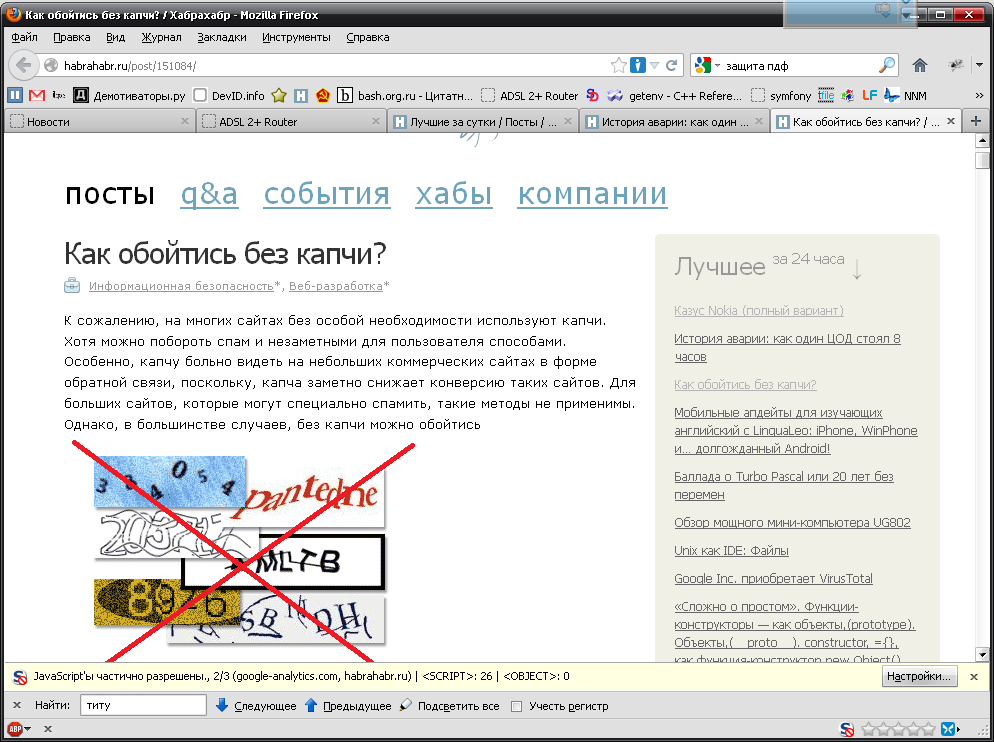
\includegraphics[scale=1,width=10cm]{ap01-09.png}
\caption{Оригінал зображення}
\label{prsc-orig:image}
\end{figure}


\begin{figure}
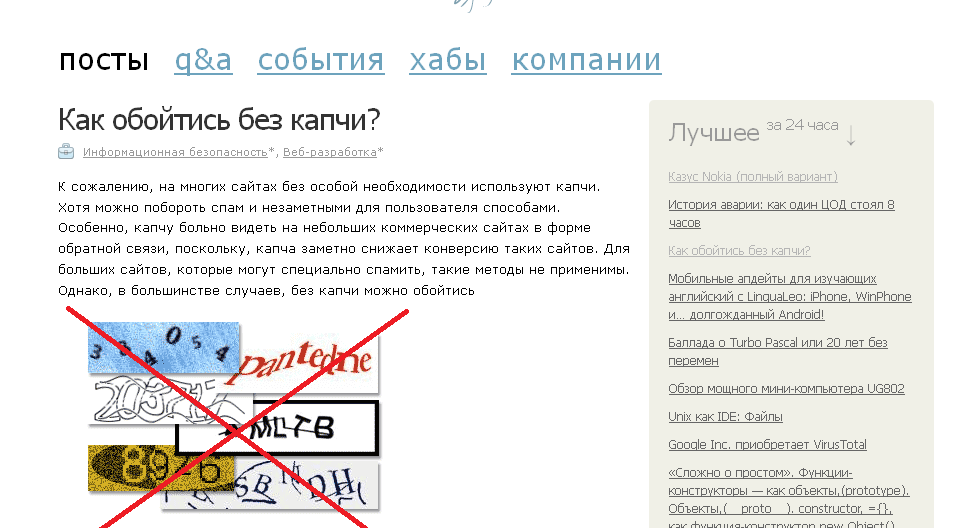
\includegraphics[scale=1,width=10cm]{ap01-10.png}
\caption{Оброблене зображення}
\label{prsc-rel:image}
\end{figure}

\begin{figure}
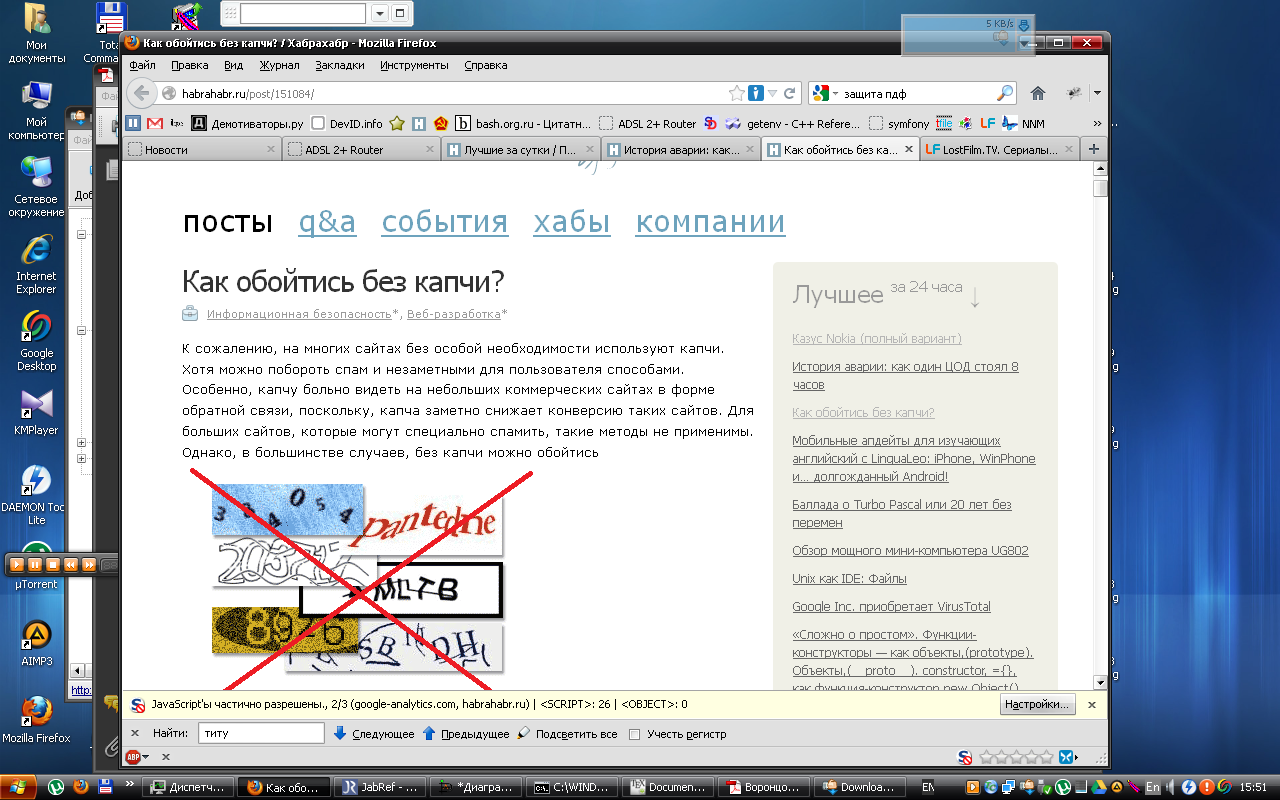
\includegraphics[scale=1,width=10cm]{ap01-11.png}
\caption{Необроблене зображення}
\label{prsc-bad:image}
\end{figure}